\documentclass[12pt]{beamer}

\setbeamertemplate{sidebar right}{}% or get rid of navigation entries there somehow
\addtobeamertemplate{footline}{\hfill\usebeamertemplate***{navigation symbols}%
	\hspace*{0.1cm}\par\vskip 2pt}{}

\AtBeginSubsection[]
{
	\begin{frame}
	\frametitle{Where are we?}
	\tableofcontents[currentsubsection]
\end{frame}
}

\usetheme{Singapore}

\usepackage[utf8]{inputenc}
\usepackage{menukeys}
\usepackage{tabularx}
\usepackage{minted}
\usepackage{makecell}
\setminted[CSS]{fontsize=\small, tabsize=2, breaklines, linenos}
\setminted[HTML]{fontsize=\small, tabsize=2, breaklines, linenos}

\title{ 
\includegraphics[width=0.5\linewidth]{hackerschool} \\ Introduction to HTML and CSS}
\author{Julius Putra Tanu Setiaji}
\date{1 September 2018}



\begin{document}

\frame{\titlepage}

\section{Introduction}
\subsection{}

\begin{frame}
\frametitle{NUS Hackers}

\begin{center}	

\includegraphics[width=0.5\linewidth]{NUSHackers}

\url{http://nushackers.org}
\end{center}

\begin{center}
	\textbf{Hacker}school
	
	Friday \textbf{Hacks}
	
	\textbf{Hack} \& Roll
	
	NUS \textbf{Hacker}space
\end{center}

\end{frame}

\begin{frame}
\frametitle{About Me}
Hi! I'm Julius. My GitHub is \url{https://github.com/indocomsoft}\\

A Year 2 Computer Science Undergraduate who loves hacking and building systems.\\

I took CS1101S taught in JavaScript and have been doing web development intensively for the past 2 years (including the Source Academy back-end and NUSSU commIT Duty Website).\\

(Not so important) I also enjoy Aerospace Engineering, Music Theory and History. {\tiny (my favourite games are KSP and EU4 hit me up if you play those too)}
\end{frame}

\begin{frame}
\frametitle{About This Workshop}
\begin{itemize}
	\item Beginner level workshop
	\item No prior knowledge assumed
	\item Static web pages
	\item Basic HTML, CSS, Framework
	\item Walk away with your own website
\end{itemize}
\end{frame}

\begin{frame}
\frametitle{Table of Contents}
\tableofcontents
\end{frame}

\begin{frame}
\frametitle{Required Software}
\begin{itemize}
	\item \textbf{Google Chrome} (\url{https://chrome.google.com/})
	\item \textbf{VS Code} (\url{https://code.visualstudio.com/}) or any decent text editor
\end{itemize}
\end{frame}

\section{HTML}
\subsection{Basic HTML}
\begin{frame}
\frametitle{Let's take a look}
\begin{center}
	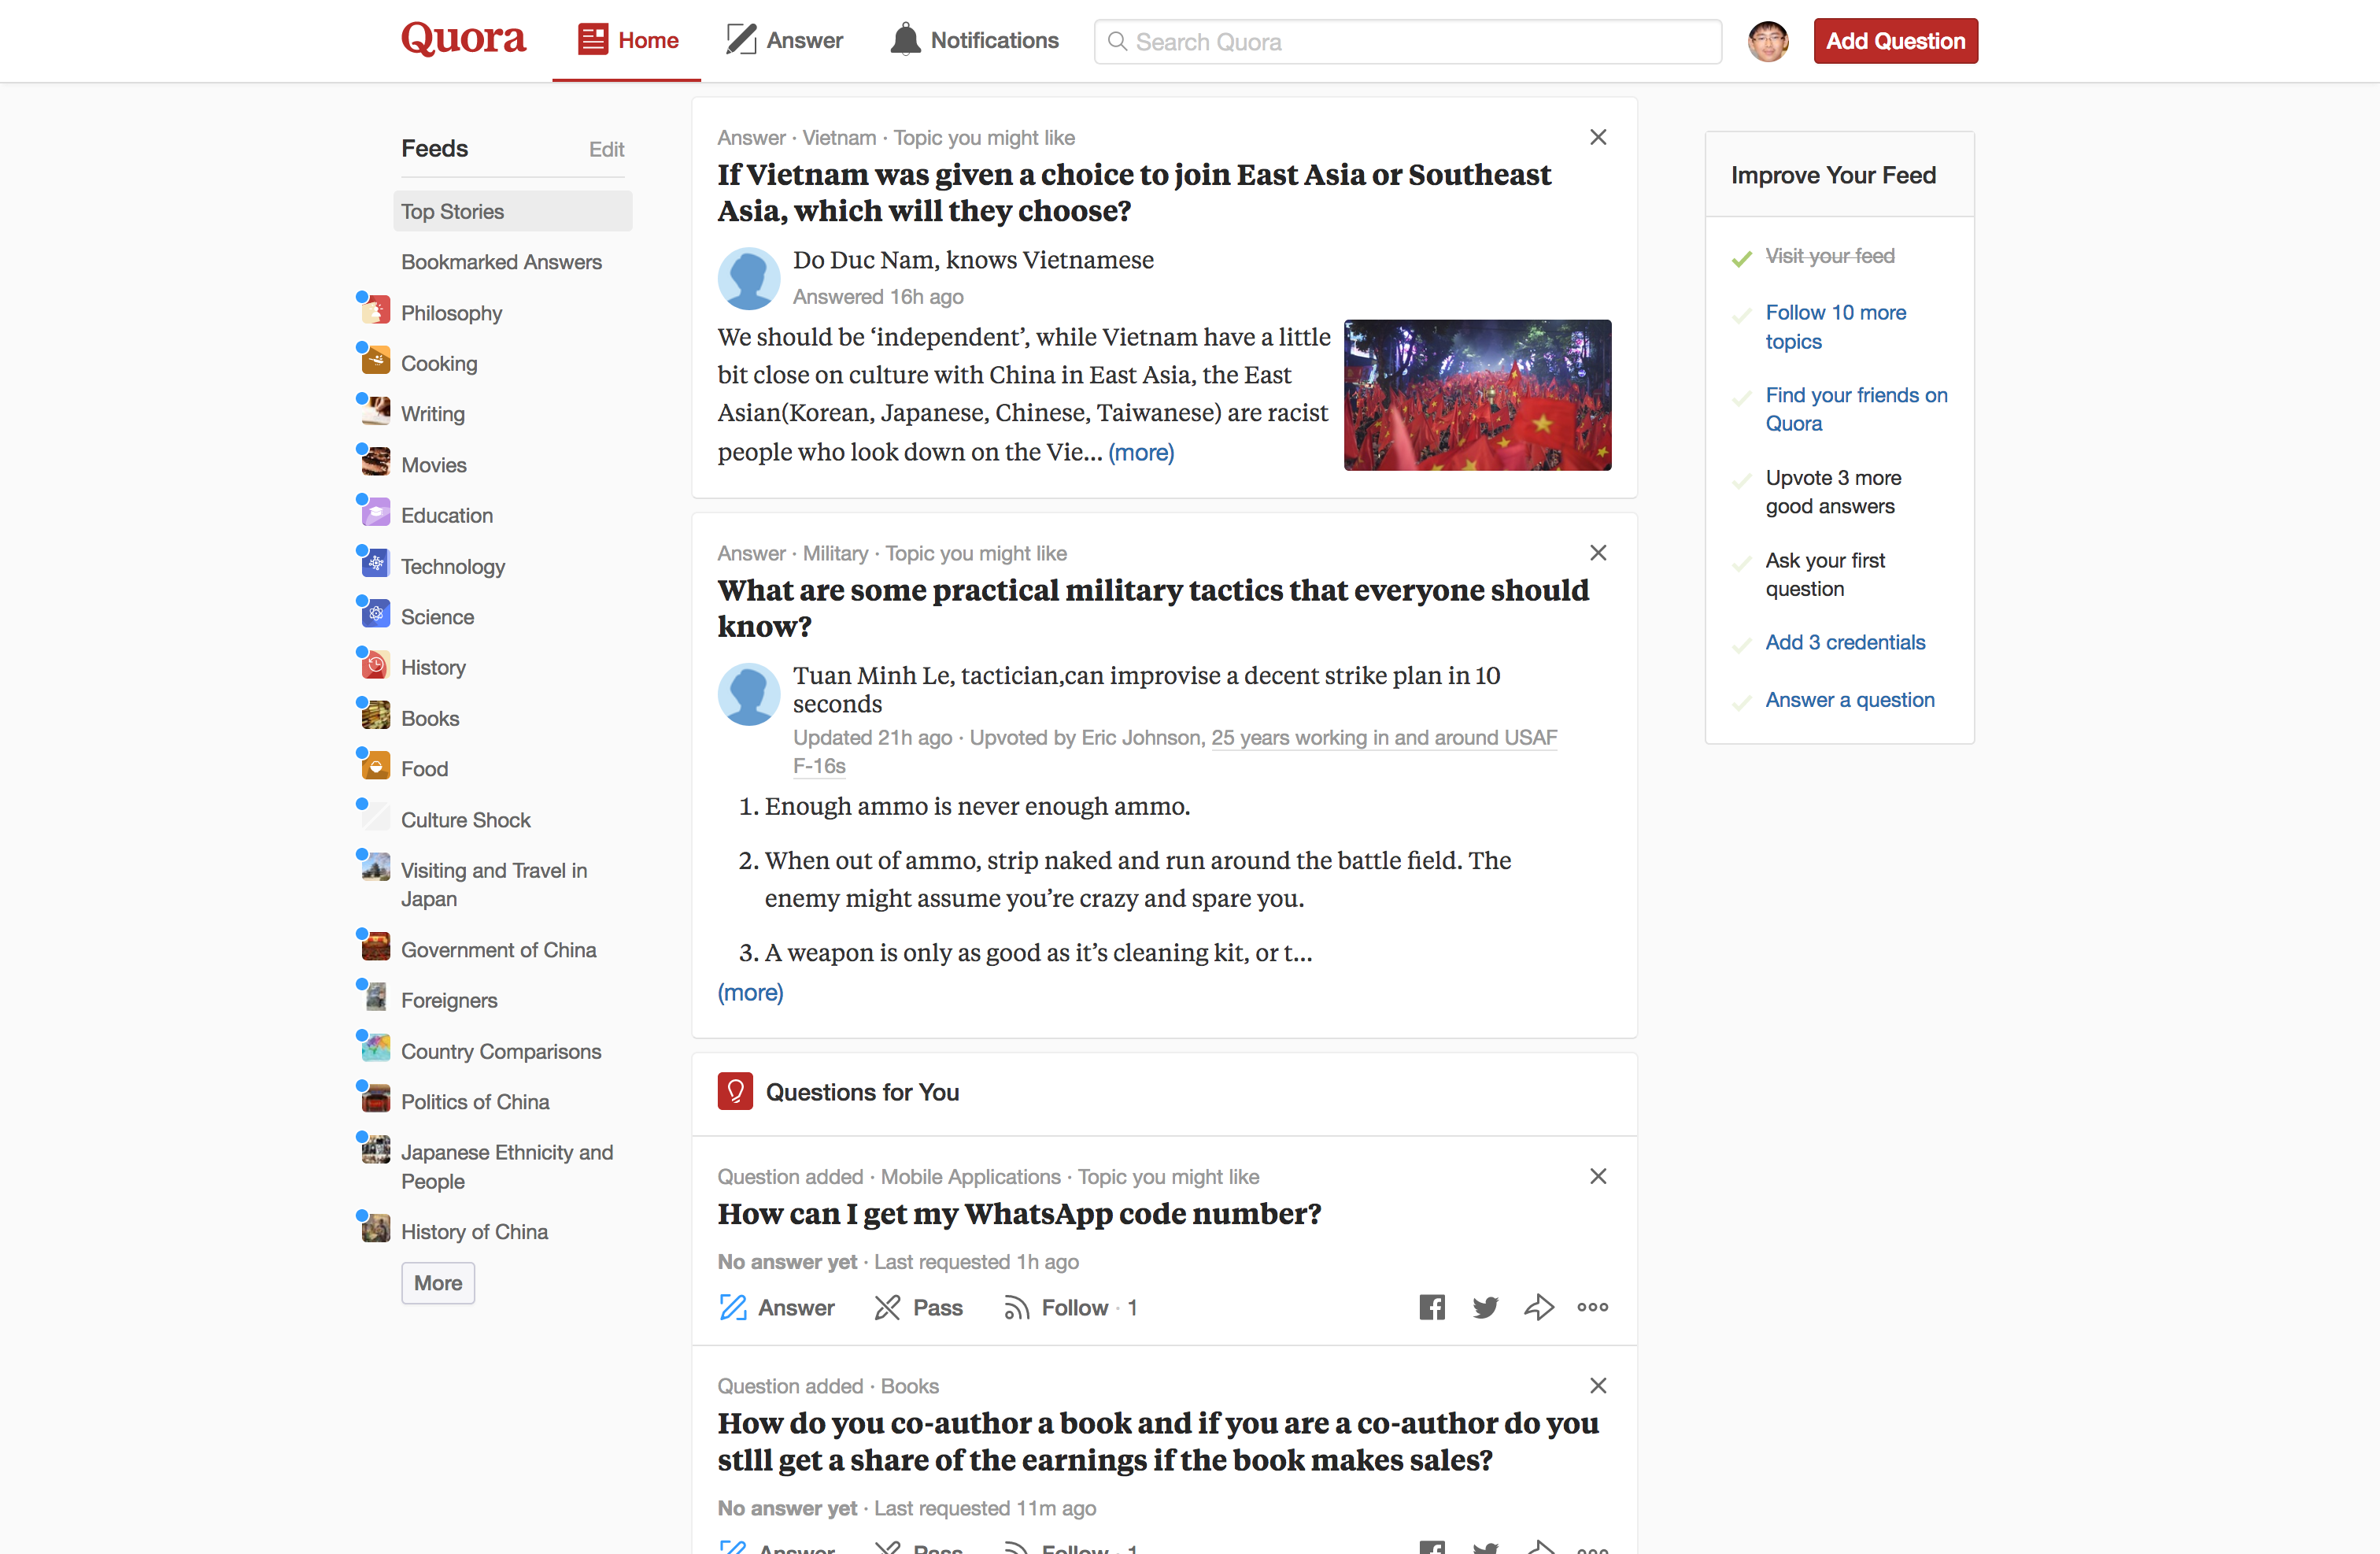
\includegraphics[width=\linewidth]{quora}
\end{center}
\end{frame}

\begin{frame}
\frametitle{Elements in a page}
\begin{columns}
	\begin{column}{0.8\linewidth}
		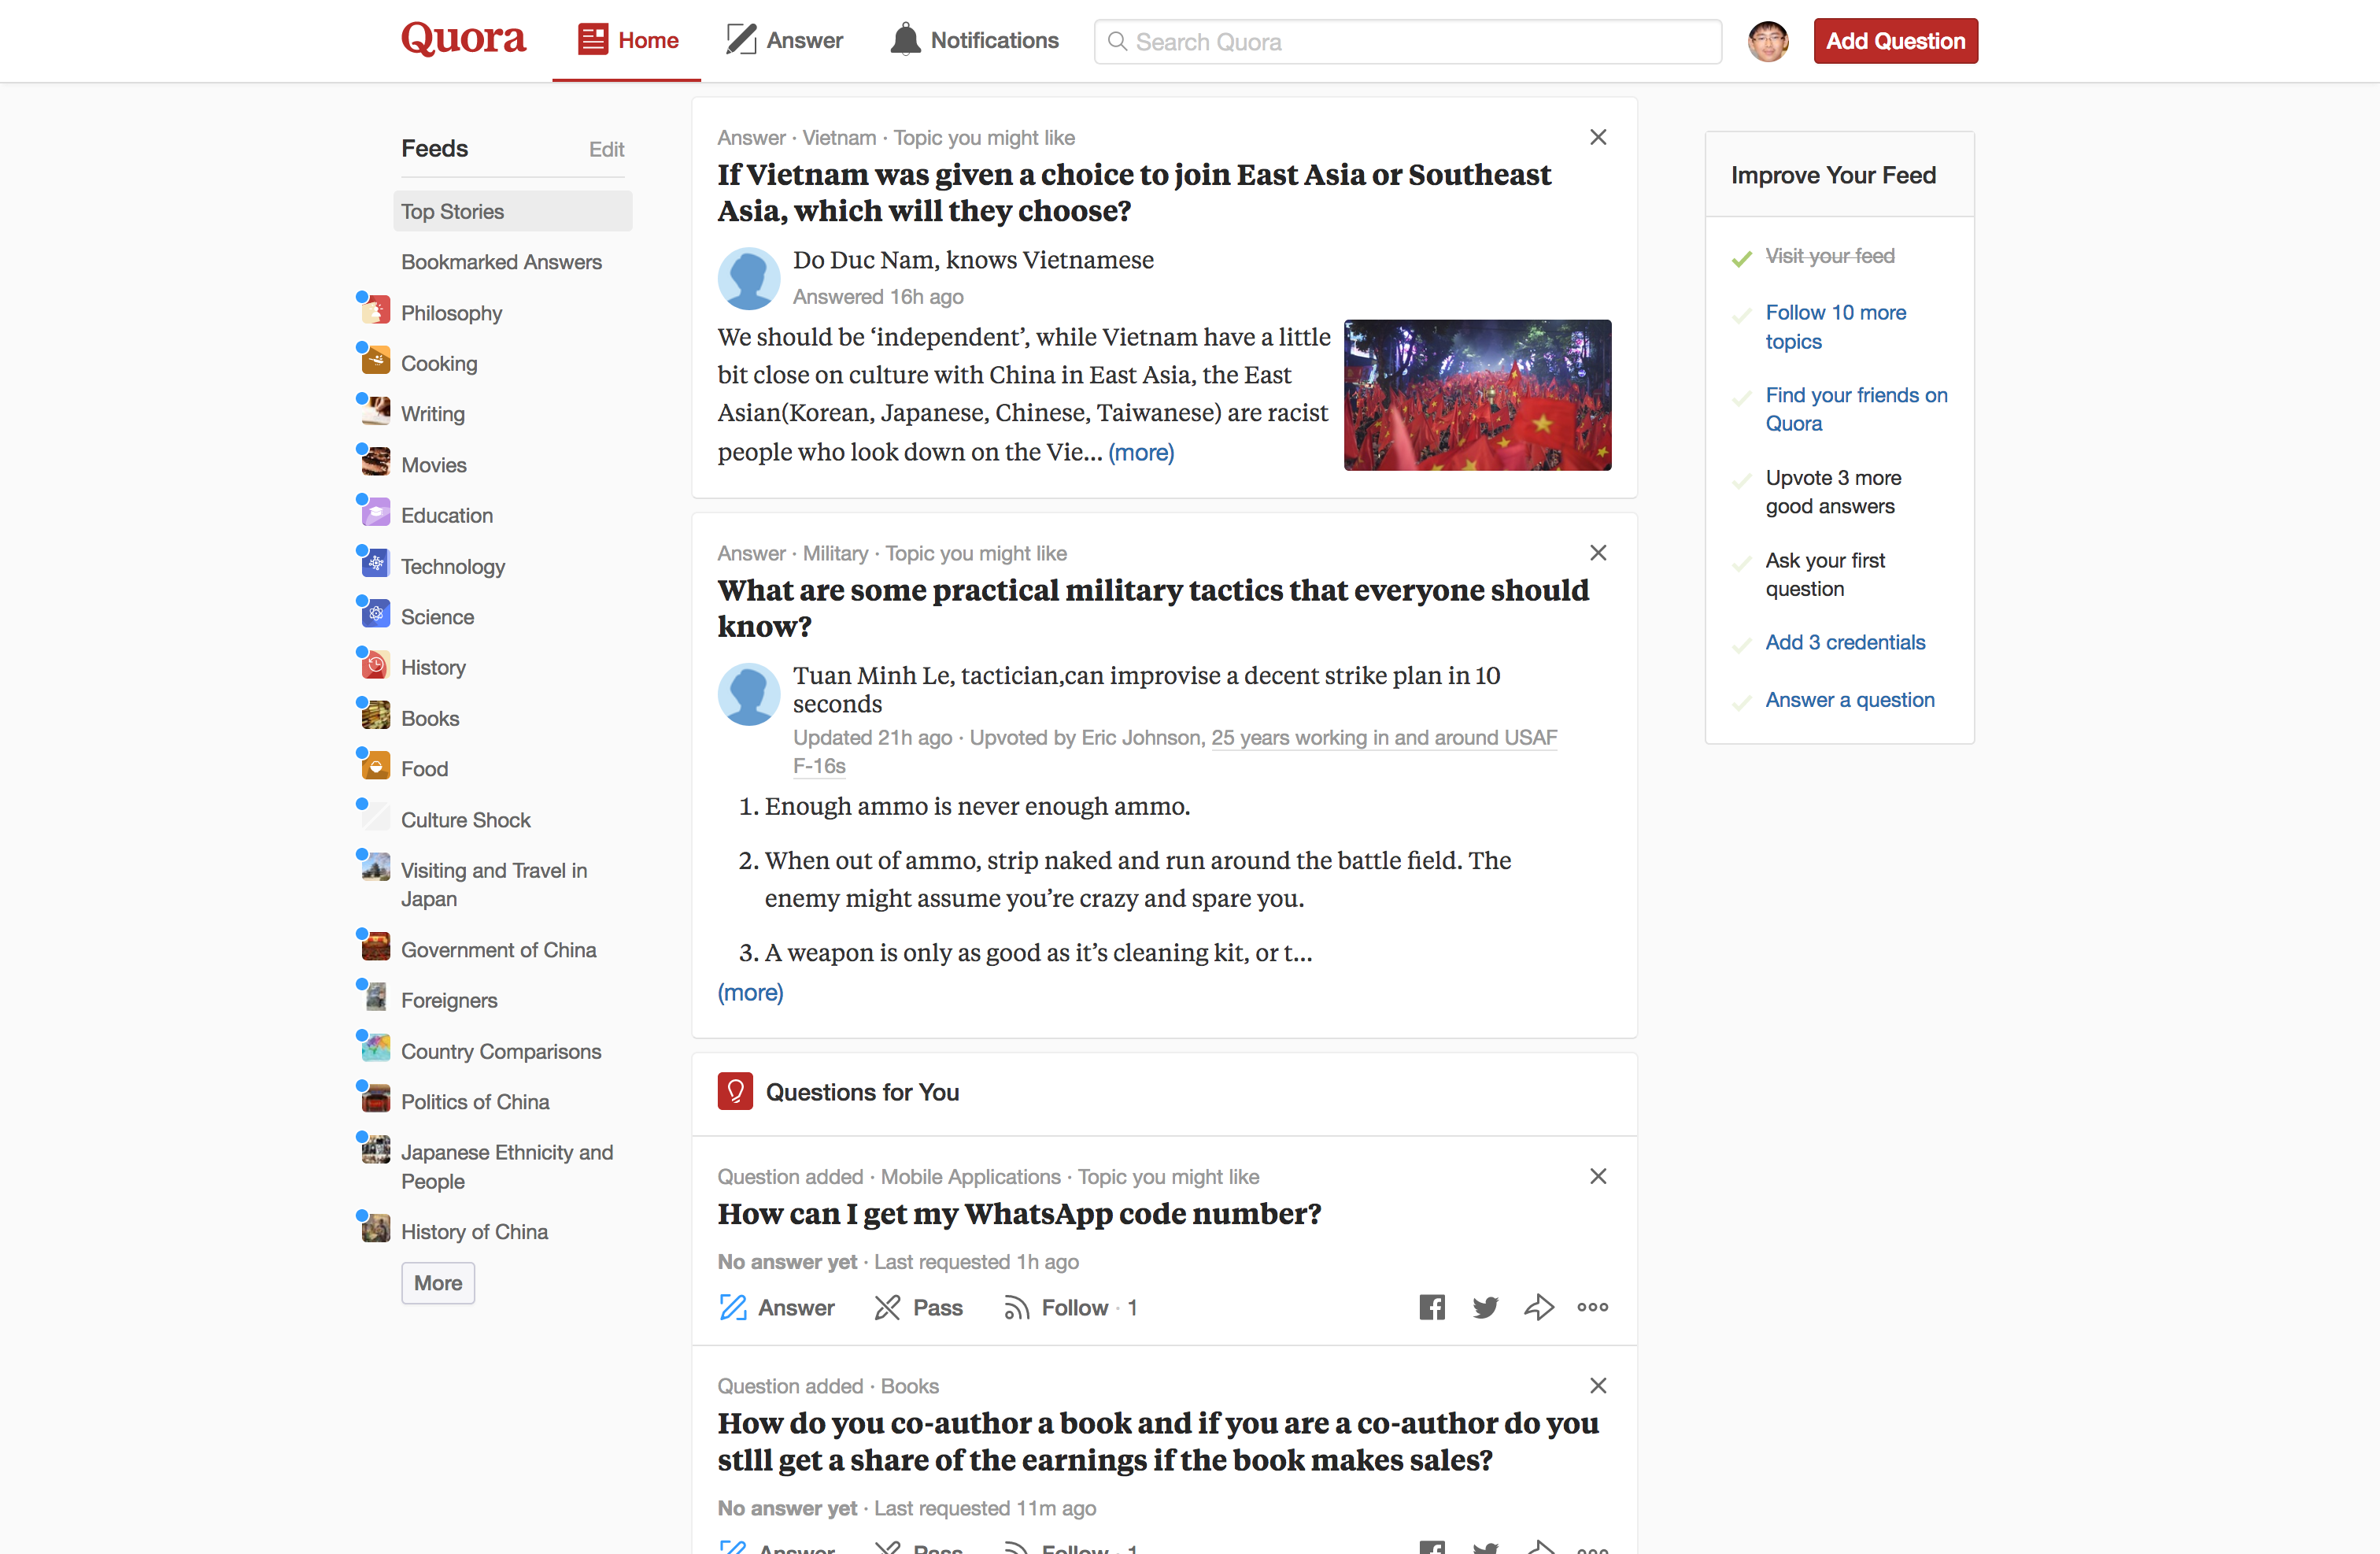
\includegraphics[width=\linewidth]{quora}
	\end{column}
	\begin{column}{0.4\linewidth}
		\begin{itemize}
			\item Navigation bar
			\item Sidebar
			\item Main content
			\item Text
			\item Image
			\item Button
		\end{itemize}
	\end{column}
\end{columns}
\end{frame}

\begin{frame}
\frametitle{HyperText Markup Language}
\begin{itemize}
	\item Standard markup language for creating web pages and web application.
	\item Markup language = a system for annotating a document.
	\item For HTML: annotations prescribing actions and presentation.
	\item First proposed by physicist Tim-Berners Lee at CERN in 1990.
	\item Currently at version 5 (HTML5)
\end{itemize}
\end{frame}

\begin{frame}
\frametitle{Let's Get the Party Started!}
\begin{enumerate}
	\item Create a directory called \texttt{workspace} on your Desktop
	\item Open VS Code and create a new file
	\item Enter your name
	\item Save as \texttt{mypage.html} inside the directory you creted
	\item Open in Chrome by drag-and-drop or double-clicking.
\end{enumerate}
\begin{columns}
	\begin{column}{0.5\linewidth}
		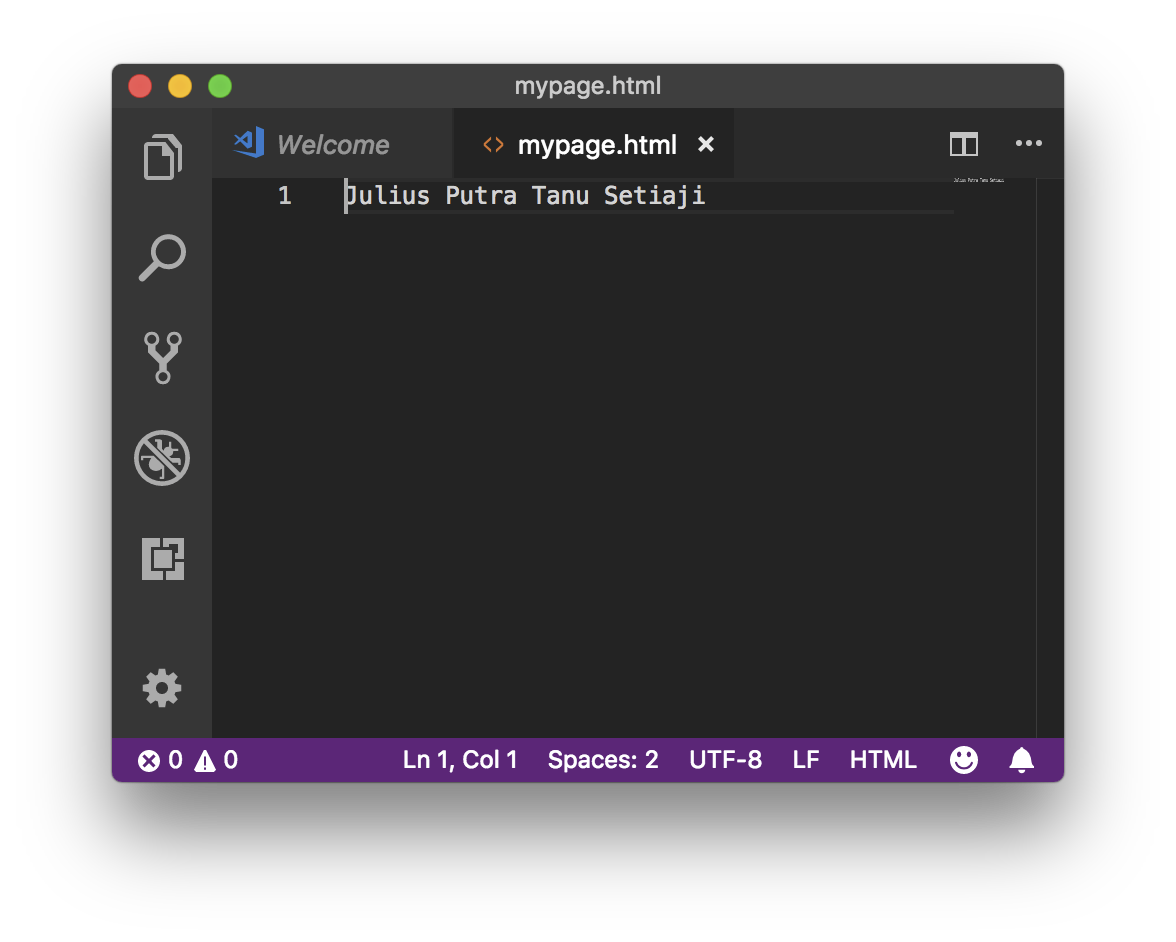
\includegraphics[width=\linewidth]{vscode-newfile}
	\end{column}
	\begin{column}{0.5\linewidth}
		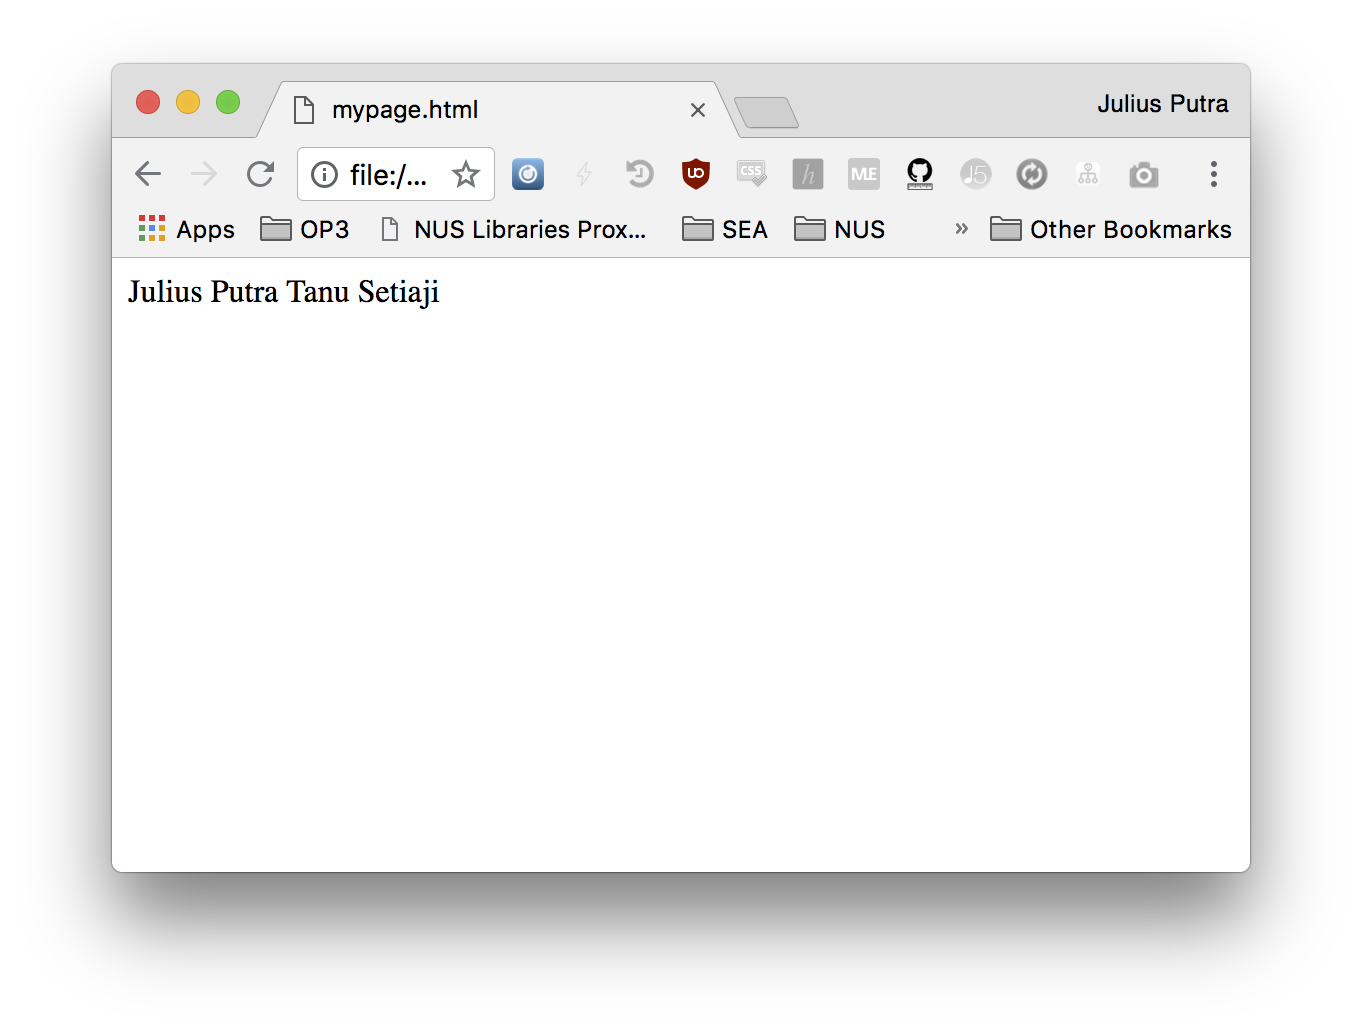
\includegraphics[width=\linewidth]{chrome-newfile}
	\end{column}
\end{columns}
\end{frame}

\begin{frame}
\frametitle{Inspecting the Webpage}
\menu{Tools > More Tools > Developer Tools} or \menu{Right click > Inspect}\\
\textbf{Keyboard Shortcut:}\\
\keys{\ctrlwin + \shift + j} or \keys{F12} (Windows), or \keys{\cmd + \Altmac + i} (Mac)
\begin{center}
	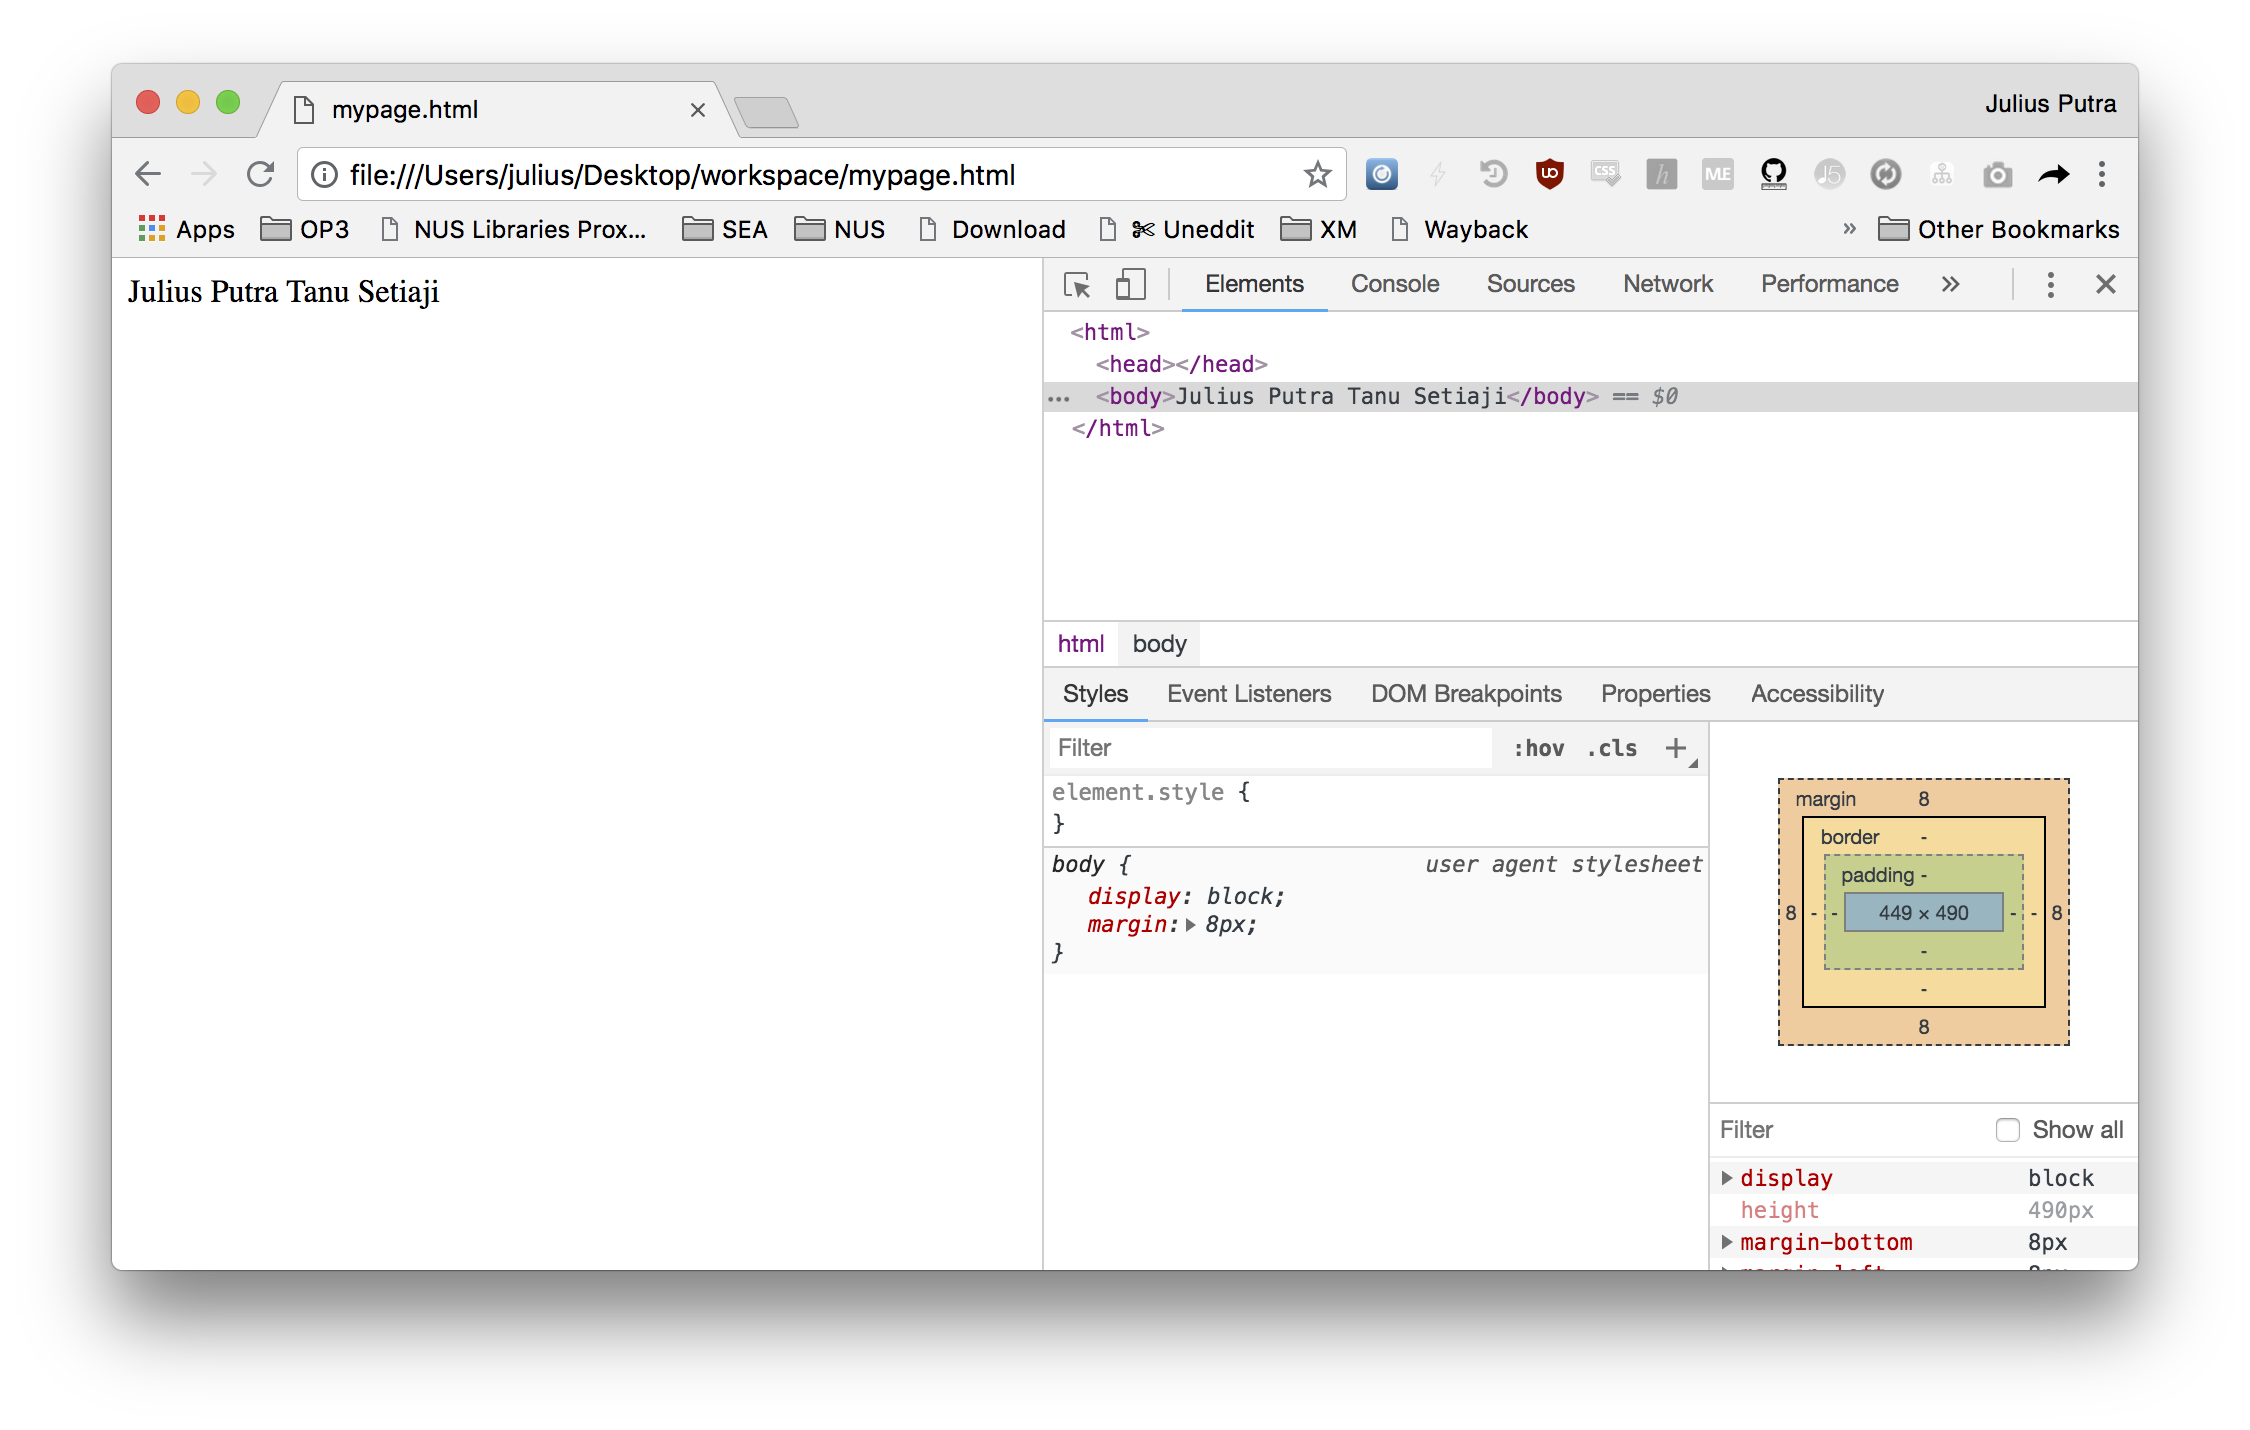
\includegraphics[width=0.75\linewidth]{devtools}
\end{center}
\end{frame}

\begin{frame}[fragile]
\frametitle{HTML Document}
\begin{minted}{HTML}
<html>
	<head></head>
	<body>hello</body>
</html>
\end{minted}
A very lenient format!
\end{frame}

\begin{frame}[fragile]
\frametitle{HTML Elements}
\begin{itemize}
	\item An element is a part of a webpage, which may contain a data item or a chunk of text or an image, or perhaps nothing \footnotemark.
	\item HTML elements can contain other elements.
\end{itemize}
\vspace{0.3cm}
\begin{columns}
	\begin{column}{0.3\linewidth}
		\begin{minted}{HTML}
<html>
	<head></head>
	<body>hello</body>
</html>
		\end{minted}
	\end{column}
	\begin{column}{0.7\linewidth}
		There are 3 HTML elements:
		\begin{enumerate}
			\item \mintinline{HTML}{<html></html>} containing 2 elements
			\item \mintinline{HTML}{<head></head>} that is empty.
			\item \mintinline{HTML}{<body></body>} containing text.
		\end{enumerate}
	\end{column}
\end{columns}

\footnotetext[1]{Taken from \url{https://developer.mozilla.org/en-US/docs/Glossary/Element}}
\end{frame}

\subsection{Basic HTML Tags}

\begin{frame}[fragile]
\frametitle{HTML Tags}
\begin{itemize}
	\item A HTML tag is used for creating an element.
	\item The name of an HTML tag is the name used in angle brackets, such as \mintinline{HTML}{<html>}\footnotemark
	\item Two types: opening \& closing tags.
	\item Closing tag is formed by adding slash to the tag name, e.g. opening: \mintinline{HTML}{<html>}, closing: \mintinline{HTML}{</html>}
\end{itemize}
\begin{columns}
	\begin{column}{0.3\linewidth}
		\begin{minted}{HTML}
		<html>
		<head></head>
		<body>hello</body>
		</html>
		\end{minted}
	\end{column}
	\begin{column}{0.5\linewidth}
		There are 6 tags. Each tag are a pair of opening and closing tags.
		\begin{itemize}
			\item \mintinline{HTML}{<html>} and \mintinline{HTML}{</html>}
			\item \mintinline{HTML}{<head>} and \mintinline{HTML}{</head>}
			\item \mintinline{HTML}{<body} and \mintinline{HTML}{</body>}
		\end{itemize}
	\end{column}
\end{columns}
\footnotetext[2]{Taken from \url{https://developer.mozilla.org/en-US/docs/Glossary/Tag}}
\end{frame}

\begin{frame}
\frametitle{The \texttt{html} tag}
\begin{itemize}
	\item Represents the top-level element of a HTML document.\footnotemark
	\item All other elements are contained inside this element.
\end{itemize}
\footnotetext[3]{Taken from \url{https://developer.mozilla.org/en-US/docs/Web/HTML/Element/html}}
\end{frame}

\begin{frame}[fragile]
\frametitle{Let's Try It Out}
\begin{minted}{HTML}
<html>
</html>
\end{minted}
\begin{enumerate}
	\item Save in VS Code (\menu{File > Save} or \keys{\ctrlwin + s} or \keys{\cmd + s})
	\item Reload in Chrome (\menu{View > Reload} or \keys{F5} or \keys{\cmd + r})
\end{enumerate}
\end{frame}

\begin{frame}
\frametitle{The \texttt{head} tag}
\begin{itemize}
	\item Provides general information (metadata) about the document, including its title and links to its scripts and style sheets.\footnotemark
\end{itemize}
\footnotetext[4]{Taken from \url{https://developer.mozilla.org/en-US/docs/Web/HTML/Element/head}}
\end{frame}

\begin{frame}
\frametitle{The \texttt{body} tag}
\begin{itemize}
	\item Represents the content of an HTML document \footnotemark
\end{itemize}
\footnotetext[5]{Taken from \url{https://developer.mozilla.org/en-US/docs/Web/HTML/Element/body}}
\end{frame}

\begin{frame}[fragile]
\frametitle{Let's Try It Out}
\begin{minted}{HTML}
<html>
	<head></head>
	<body></body>
</html>
\end{minted}
\begin{enumerate}
	\item Save in VS Code (\menu{File > Save} or \keys{\ctrlwin + s} or \keys{\cmd + s})
	\item Reload in Chrome (\menu{View > Reload} or \keys{F5} or \keys{\cmd + r})
\end{enumerate}
\end{frame}

\begin{frame}
\frametitle{The \texttt{title} tag}
\begin{itemize}
	\item Defines the document's title\footnotemark
	\item Shown in a browser's title bar or a page's tab.
	\item Must be put inside \mintinline{HTML}{<head></head>}
\end{itemize}
\footnotetext[6]{Taken from \url{https://developer.mozilla.org/en-US/docs/Web/HTML/Element/title}}
\end{frame}

\begin{frame}[fragile]
\frametitle{Let's Try It Out}
\begin{minted}{HTML}
<html>
	<head>
		<title>My First Page!</title>
	</head>
	<body></body>
</html>
\end{minted}
\begin{enumerate}
	\item Save in VS Code (\menu{File > Save} or \keys{\ctrlwin + s} or \keys{\cmd + s})
	\item Reload in Chrome (\menu{View > Reload} or \keys{F5} or \keys{\cmd + r})
\end{enumerate}
\end{frame}

\begin{frame}
\frametitle{The \texttt{p} tag}
\begin{itemize}
	\item Represents a paragraph of text \footnotemark
	\item Represented in visual media as blocks of text that are separated from adjacent blocks.
\end{itemize}
\footnotetext[6]{Taken from \url{https://developer.mozilla.org/en-US/docs/Web/HTML/Element/p}}
\end{frame}

\begin{frame}[fragile]
\frametitle{Let's Try It Out}
\begin{minted}{HTML}
<html>
	<head>
		<title>My First Page!</title>
	</head>
	<body>
		<p>Hello, world!</p>
	</body>
</html>
\end{minted}
\begin{enumerate}
	\item Save in VS Code (\menu{File > Save} or \keys{\ctrlwin + s} or \keys{\cmd + s})
	\item Reload in Chrome (\menu{View > Reload} or \keys{F5} or \keys{\cmd + r})
\end{enumerate}
\end{frame}

\begin{frame}
\frametitle{The \texttt{h[1-6]} tag}
\begin{itemize}
	\item Represents section headings.\footnotemark
	\item There are 6 levels of hierarchy with 1 being the largest and so on:
	\begin{itemize}
		\item \mintinline{HTML}{<h1></h1>}
		\item \mintinline{HTML}{<h2></h2>}
		\item \mintinline{HTML}{<h3></h3>}
		\item \mintinline{HTML}{<h4></h4>}
		\item \mintinline{HTML}{<h5></h5>}
		\item \mintinline{HTML}{<h6></h6>}
	\end{itemize}
\end{itemize}
\footnotetext[6]{Taken from \url{https://developer.mozilla.org/en-US/docs/Web/HTML/Element/Heading_Elements}}
\end{frame}

\begin{frame}[fragile]
\frametitle{Let's Try It Out}
\begin{minted}[firstnumber=5]{HTML}
	<body>
		<h1>Julius</h1>
		<p>Hello, world!</p>
		<h2>About me</h2>
		<h2>Hobbies</h2>
		<h2>Websites</h2>
	</body>
\end{minted}
\begin{enumerate}
	\item Save in VS Code (\menu{File > Save} or \keys{\ctrlwin + s} or \keys{\cmd + s})
	\item Reload in Chrome (\menu{View > Reload} or \keys{F5} or \keys{\cmd + r})
\end{enumerate}
\end{frame}

\subsection{Attribute}

\begin{frame}[fragile]
\frametitle{Attribute}
\begin{itemize}
	\item An attribute extends a tag, changing its behavior or providing metadata\footnotemark
	\item Less cheem: It provides additional information about the tag.
	\item It is defined inside the tag, with format \texttt{key=value}
	\item E.g. \mintinline{HTML}{<p align="right">Hello!</p>}
\end{itemize}
\footnotetext[7]{Taken from \url{https://developer.mozilla.org/en-US/docs/Glossary/Attribute}}
\end{frame}

\begin{frame}[fragile]
\frametitle{Let's Try It Out}
\begin{minted}[firstnumber=5]{HTML}
	<body>
		<h1>Julius</h1>
		<p align="right">Hello, world!</p>
		<h2>About me</h2>
		<h2>Hobbies</h2>
		<h2>Websites</h2>
	</body>
\end{minted}
\begin{enumerate}
	\item Save in VS Code (\menu{File > Save} or \keys{\ctrlwin + s} or \keys{\cmd + s})
	\item Reload in Chrome (\menu{View > Reload} or \keys{F5} or \keys{\cmd + r})
\end{enumerate}
\end{frame}

\begin{frame}
\frametitle{The \texttt{a} tag}
\begin{itemize}
	\item Creates a hyperlink to other web pages, files, locations\footnotemark
	\item Important attribute(s):
	\begin{itemize}
		\item \texttt{href}: Contains a URL or a URL fragment that the hyperlink points to.
		\item \texttt{target}: Specifies where to display the linked URL. For example, \texttt{\_blank} to load in new tab/window.
	\end{itemize}
\end{itemize}
\footnotetext[6]{Taken from \url{https://developer.mozilla.org/en-US/docs/Web/HTML/Element/a}}
\end{frame}

\begin{frame}[fragile]
\frametitle{Let's Try It Out}
\begin{minted}[firstnumber=5]{HTML}
	<body>
		<a href="http://google.com/">Google</a>
		<a href="http://google.com/" target="_blank">Google in new tab</a>
	</body>
\end{minted}
\begin{enumerate}
	\item Save in VS Code (\menu{File > Save} or \keys{\ctrlwin + s} or \keys{\cmd + s})
	\item Reload in Chrome (\menu{View > Reload} or \keys{F5} or \keys{\cmd + r})
\end{enumerate}
\end{frame}

\begin{frame}
\frametitle{The \texttt{img} tag}
\begin{itemize}
	\item Embeds an image into the document.\footnotemark
	\item A self-closing tag: \mintinline{HTML}{<img src="logo.png" alt="NUS" />}
	\item Important attribute(s):
	\begin{itemize}
		\item \texttt{src}: The image URL to embed.
		\item \texttt{alt}: An alternative text description of the image
	\end{itemize}
\end{itemize}
\footnotetext{Taken from \url{https://developer.mozilla.org/en-US/docs/Web/HTML/Element/img}}
\end{frame}

\begin{frame}[fragile]
\frametitle{Let's Try It Out}
\begin{minted}[firstnumber=5]{HTML}
	<body>
		<img src="image url" alt="description" />
	</body>
\end{minted}
\begin{enumerate}
	\item Save in VS Code (\menu{File > Save} or \keys{\ctrlwin + s} or \keys{\cmd + s})
	\item Reload in Chrome (\menu{View > Reload} or \keys{F5} or \keys{\cmd + r})
\end{enumerate}
\end{frame}

\begin{frame}
\frametitle{HTML Summary}
We learnt about:
\begin{columns}
	\begin{column}{0.5\textwidth}
		\begin{itemize}
			\item \mintinline{HTML}{<html></html>}
			\item \mintinline{HTML}{<head></head>}
			\item \mintinline{HTML}{<body></body>}
			\item \mintinline{HTML}{<h1></h1>}
			\item \mintinline{HTML}{<h2></h2>}
			\item \mintinline{HTML}{<p></p>}
			\item \mintinline{HTML}{<a></a>}
			\item \mintinline{HTML}{<img />}
		\end{itemize}
	\end{column}
	\begin{column}{0.5\textwidth}
		\begin{itemize}
			\item Element
			\item Tag
			\item Attribute
		\end{itemize}
	\end{column}
\end{columns}
You can read up more on Mozilla Developer Network (MDN): \url{https://developer.mozilla.org/en-US/docs/Web/HTML/Element}
\end{frame}

\begin{frame}
\frametitle{Break}

\includegraphics[width=\linewidth]{break}
\end{frame}

\section{CSS}
\subsection{Basic CSS}
\begin{frame}
\frametitle{Cascading Style Sheets}
\begin{itemize}
	\item Used for describing the presentation of a document written in a markup language like HTML.
	\item Designed to enable the separation of presentation and content.
	\item First released in 1996.
	\item Currently at version 3.
\end{itemize}
\end{frame}

\begin{frame}
\frametitle{On the developer console}
\begin{center}
	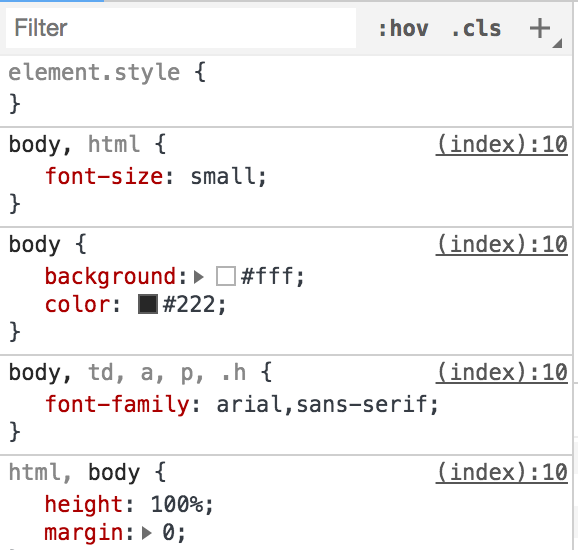
\includegraphics[width=0.7\linewidth]{css-devconsole}
\end{center}
\end{frame}

\begin{frame}[fragile]
\frametitle{Property-Value}
\begin{minted}{CSS}
color: white;
background: black;
\end{minted}
Format:\\
\texttt{property: value;}
\begin{itemize}
	\item Colon to separate between property and value.
	\item Semicolon to separate between pairs of property-value.
\end{itemize}
\end{frame}

\begin{frame}[fragile]
\frametitle{Inline Styling}
\begin{minted}[firstnumber=6]{HTML}
		<p style="background: blue;">Hello!</p>
\end{minted}
\begin{enumerate}
	\item Save in VS Code (\menu{File > Save} or \keys{\ctrlwin + s} or \keys{\cmd + s})
	\item Reload in Chrome (\menu{View > Reload} or \keys{F5} or \keys{\cmd + r})
\end{enumerate}
\end{frame}

\begin{frame}
\frametitle{The \texttt{style} tag}
\begin{itemize}
	\item Contains the CSS (styling) for a document\footnotemark
	\item Must be put inside the \texttt{head} element
\end{itemize}
\footnotetext{Taken from \url{https://developer.mozilla.org/en-US/docs/Web/HTML/Element/stle}}
\end{frame}

\begin{frame}
\frametitle{CSS Selectors}
\begin{itemize}
	\item Define the elements to which a set of CSS rules apply.\footnotemark
	\item Basic selectors:
	\begin{itemize}
		\item \textbf{Type selector}
		\item \textbf{Class selector}
		\item id selector
		\item Universal selector
		\item Attribute selector
	\end{itemize}
\end{itemize}
\footnotetext{Taken from \url{https://developer.mozilla.org/en-US/docs/Web/CSS/CSS_Selectors}}
\end{frame}

\begin{frame}[fragile]
\frametitle{Selector and Declaration Block}
\begin{minted}{CSS}
a {
	color: white;
	background: black;
}
\end{minted}
Format:
\begin{verbatim}
selector {
  property: value;
}
\end{verbatim}
\begin{itemize}
	\item Declaration block is contained inside opening and closing curly braces.
	\item List of pairs of property-value is located inside the declaration block.
	\item Selector is located before the opening curly braces.
\end{itemize}
\end{frame}

\begin{frame}[fragile]
\frametitle{Type Selector}
Matches elements by its name. Selector is just the element name.
\begin{minted}[firstnumber=2]{HTML}
<head>
	<style>
		a {
			color: red;
		}
	</style>
</head>
<body>
	<a href="http://google.com/">Google</a>
</body>
\end{minted}
\end{frame}


%\begin{frame}[fragile]
%\frametitle{Class and id}
%\begin{minted}[firstnumber=6]{HTML}
%<p class="text">Hello, world!</p>
%<p id="paragraph-2">Lorem ipsum dolor sit amet</p>
%\end{minted}
%Both class \& id are used as a "hook" in order to modify styles of elements.
%\end{frame}

%\begin{frame}[fragile]
%\frametitle{Class vs id}
%Difference\footnotemark:\\
%\begin{tabularx}{\linewidth}{|X|X|}
%\hline
%\textbf{id} & \textbf{class} \\ \hline
%Each element can have only one \texttt{id}. & Each element can have multiple classes. \\ \hline
%\texttt{id} is unique within the same document. & Each class can be used multiple times in the same document. \\ \hline
%\end{tabularx}
%\footnotetext{Taken from \url{https://css-tricks.com/the-difference-between-id-and-class/}}
%\end{frame}

\begin{frame}[fragile]
\frametitle{Class Selector}
Matches by class. Selector is by adding a full-stop before the class name.
\begin{minted}[firstnumber=2]{HTML}
<head>
	<style>
		.important {
			color: red;
		}
	</style>
</head>
<body>
	<p>Welcome to my page</p>
	<p class="important">I will be away for 2 weeks</p>
</body>
\end{minted}
\end{frame}

\begin{frame}
\frametitle{CSS Specifity}
What if I use both inline styling and the \texttt{style} tag?
\begin{itemize}
	\item If there are conflicting rules, priority is based on certain criteria.
	\item More information on \url{https://developer.mozilla.org/en-US/docs/Web/CSS/Specificity}
\end{itemize}
\end{frame}

\begin{frame}
\frametitle{CSS Summary}
We learnt about:
\begin{itemize}
	\item Property-Value
	\item Inline Styling
	\item The \texttt{style} tag
	\item CSS selectors
	\item Declaration block
\end{itemize}
You can read up more on Mozilla Developer Network (MDN): \url{https://developer.mozilla.org/en-US/docs/Web/HTML/Element}
\end{frame}

\section{Bootstrap Framework}
\subsection{Introduction}
\begin{frame}
\frametitle{Introduction to Bootstrap Framework}
\begin{center}
	\url{http://getbootstrap.com}
	
	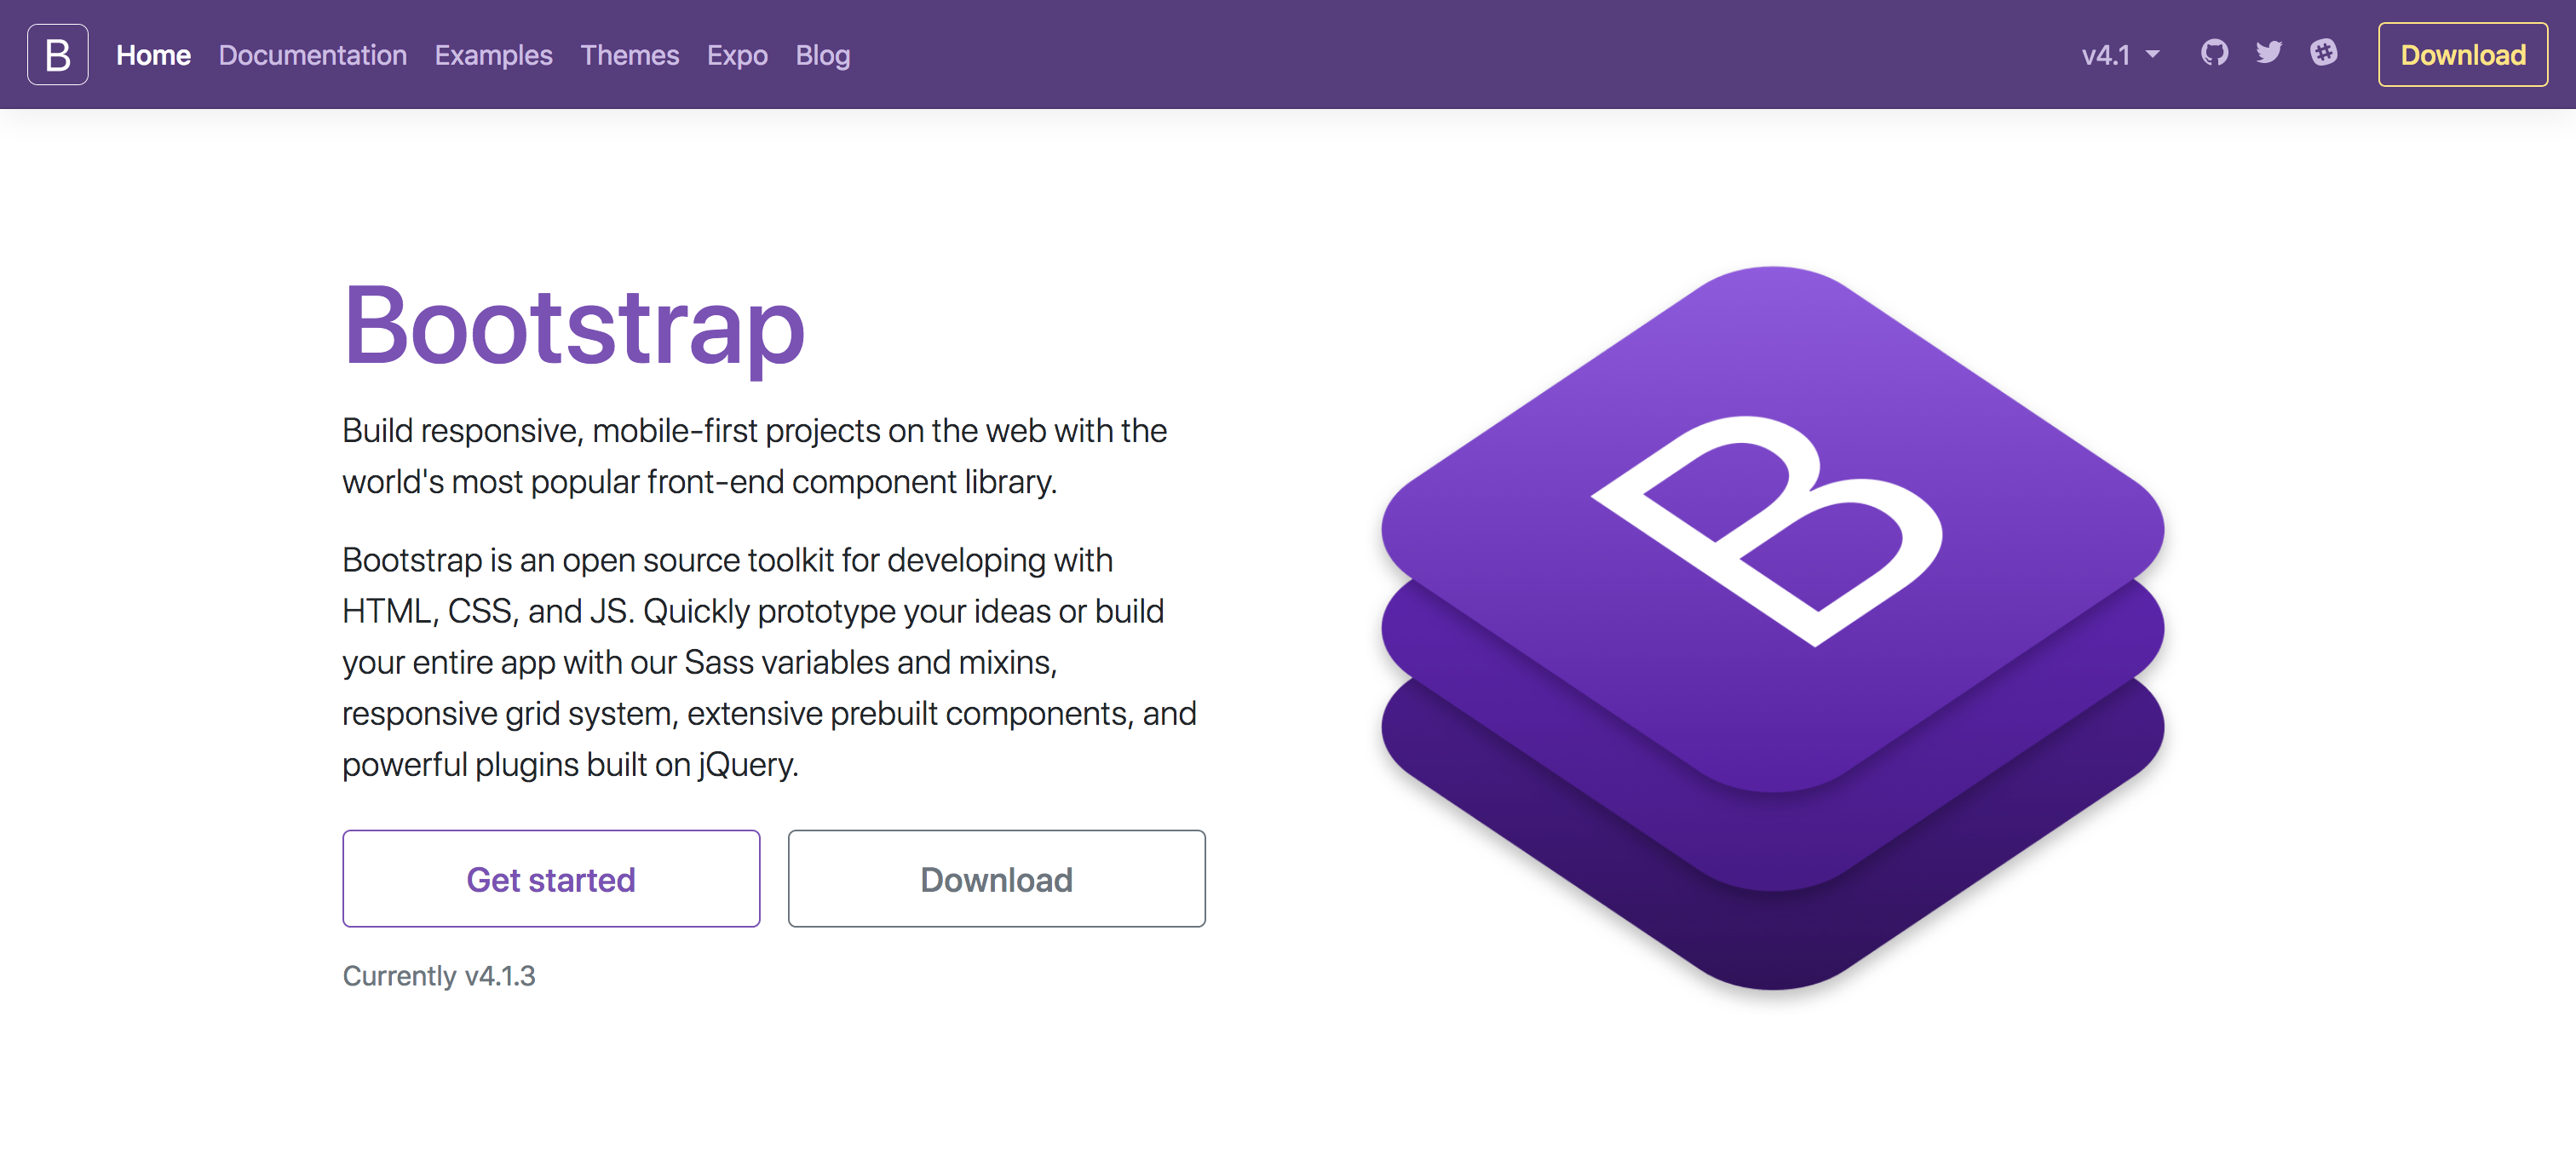
\includegraphics[width=\linewidth]{bootstrap}
\end{center}
\end{frame}

\begin{frame}
\frametitle{Using Bootstrap}
Copy and paste starter template from
\url{http://getbootstrap.com/docs/4.1/getting-started/introduction/\#starter-template}
\end{frame}

\begin{frame}
\frametitle{Revisiting Quora}
\begin{center}
	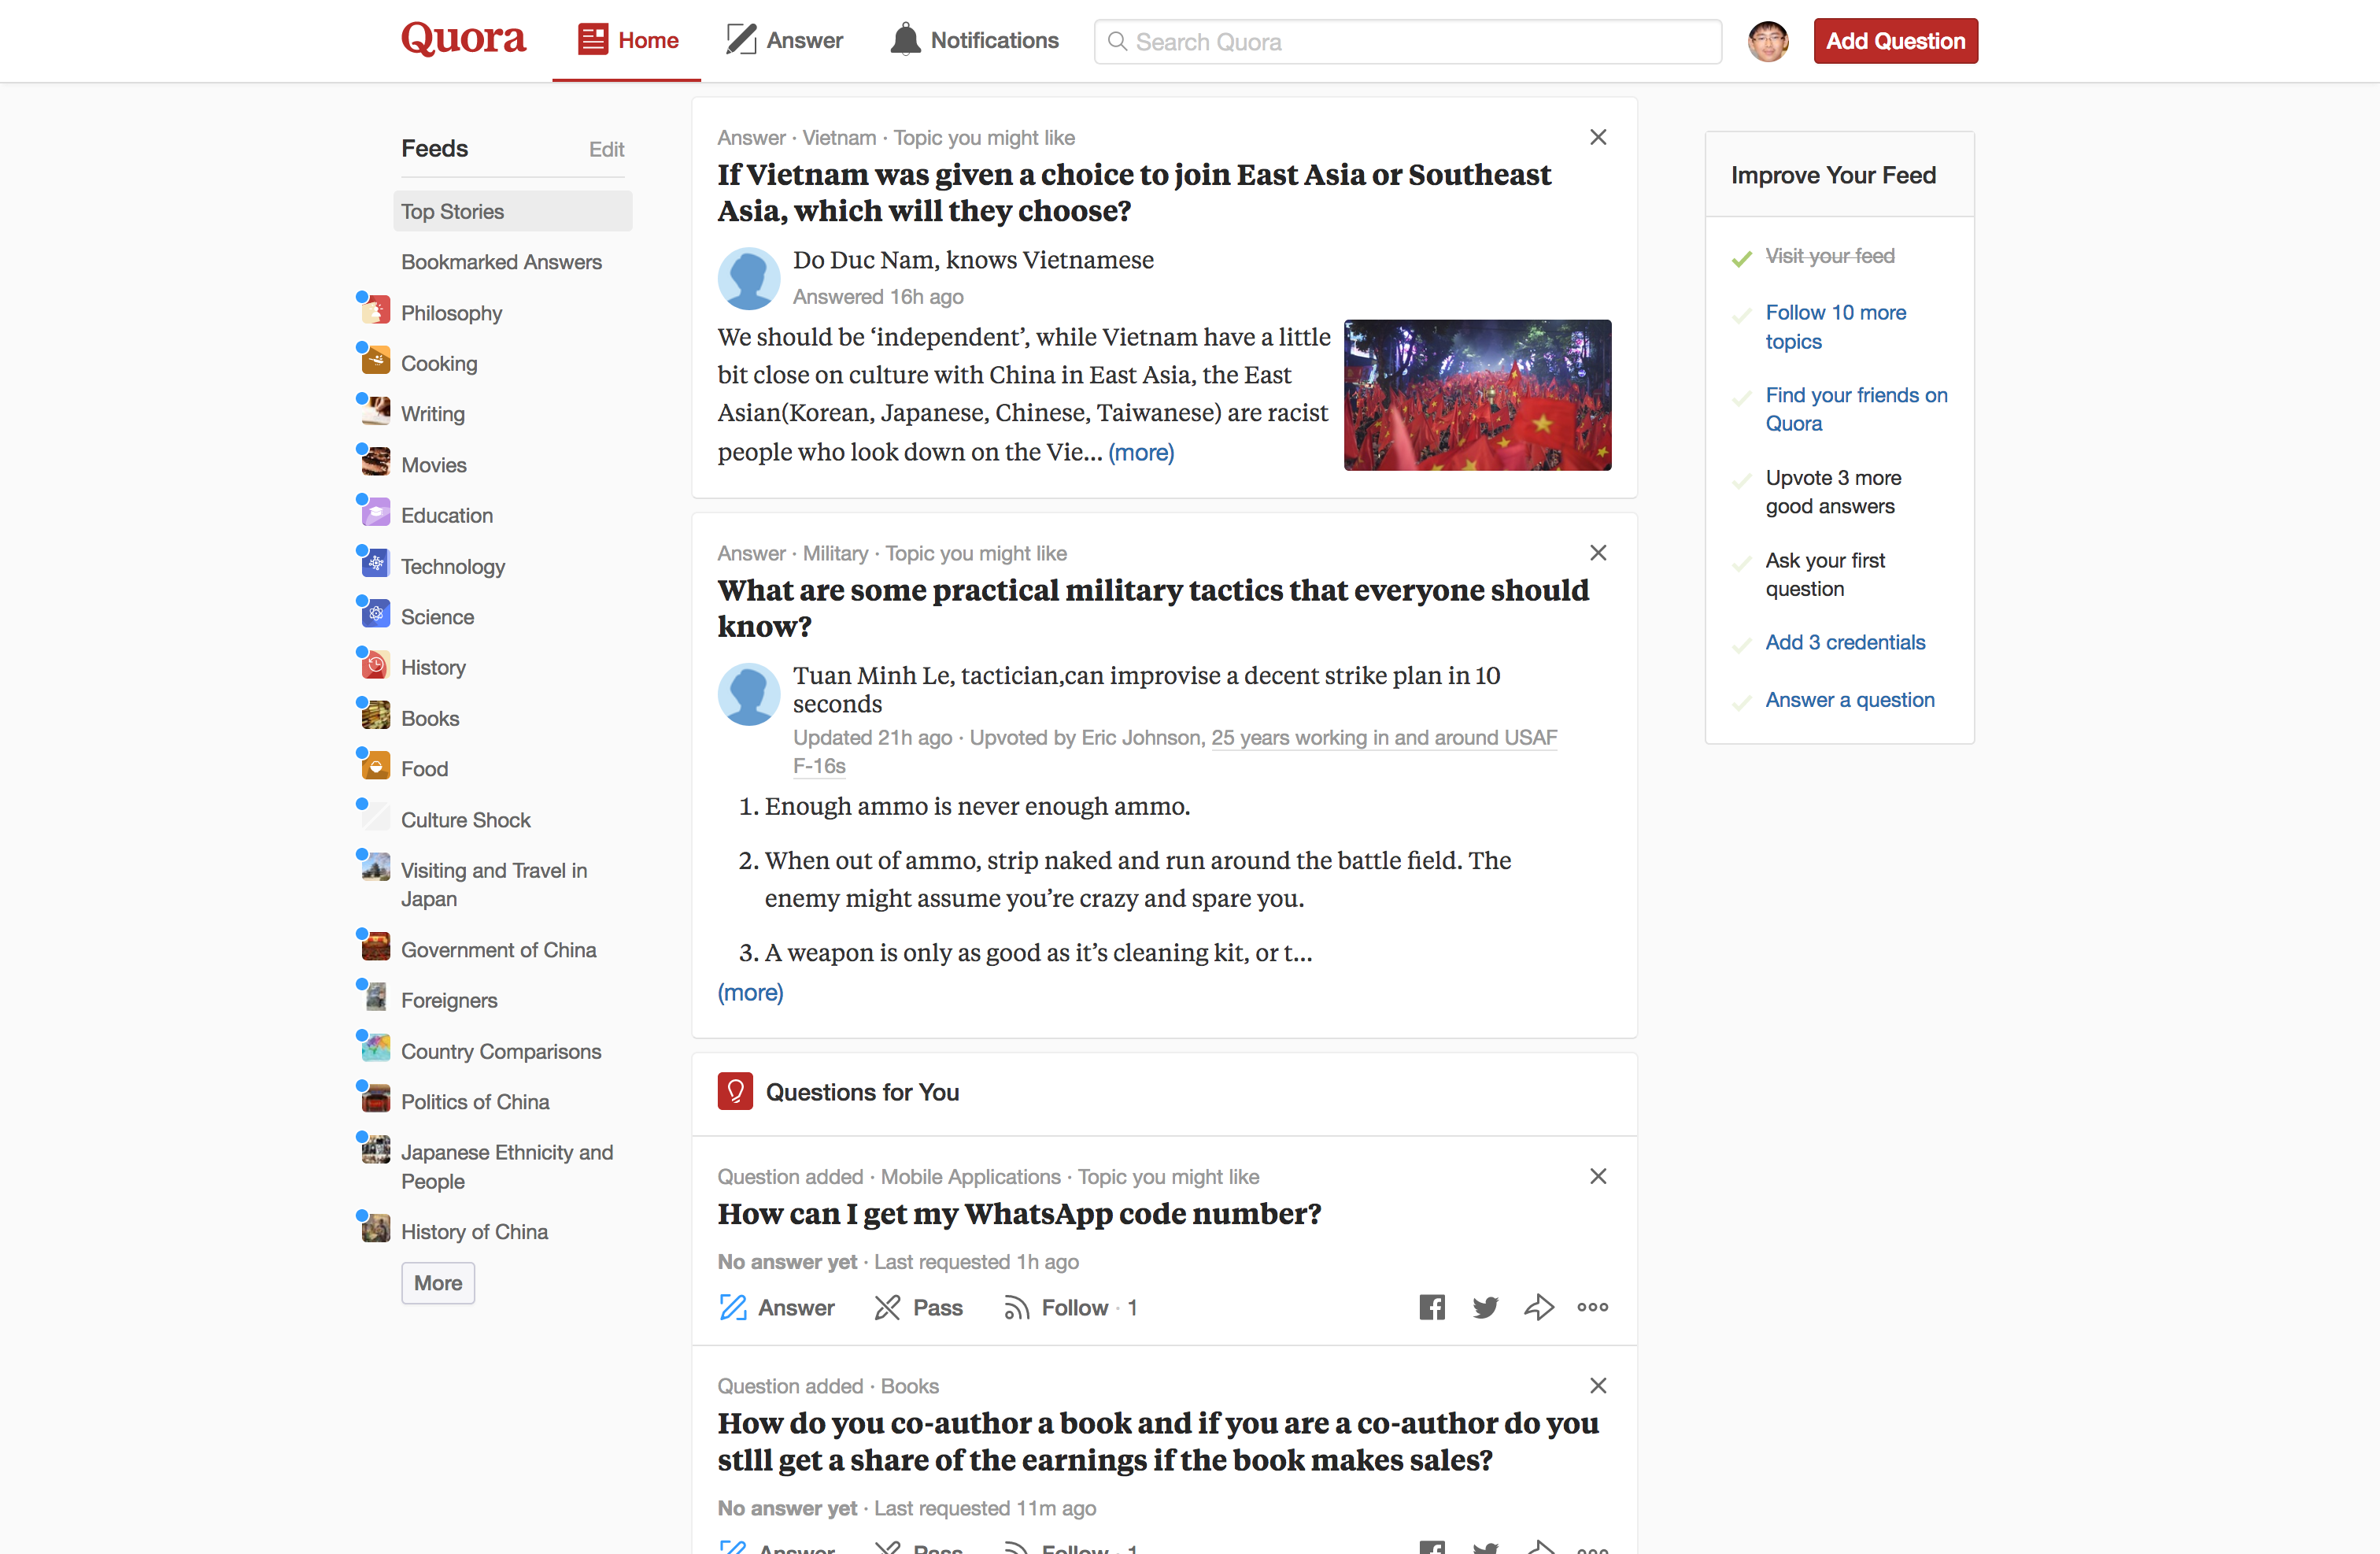
\includegraphics[width=\linewidth]{quora}
\end{center}
\end{frame}

\begin{frame}
\frametitle{Bootstrap Layouting}
\begin{center}
	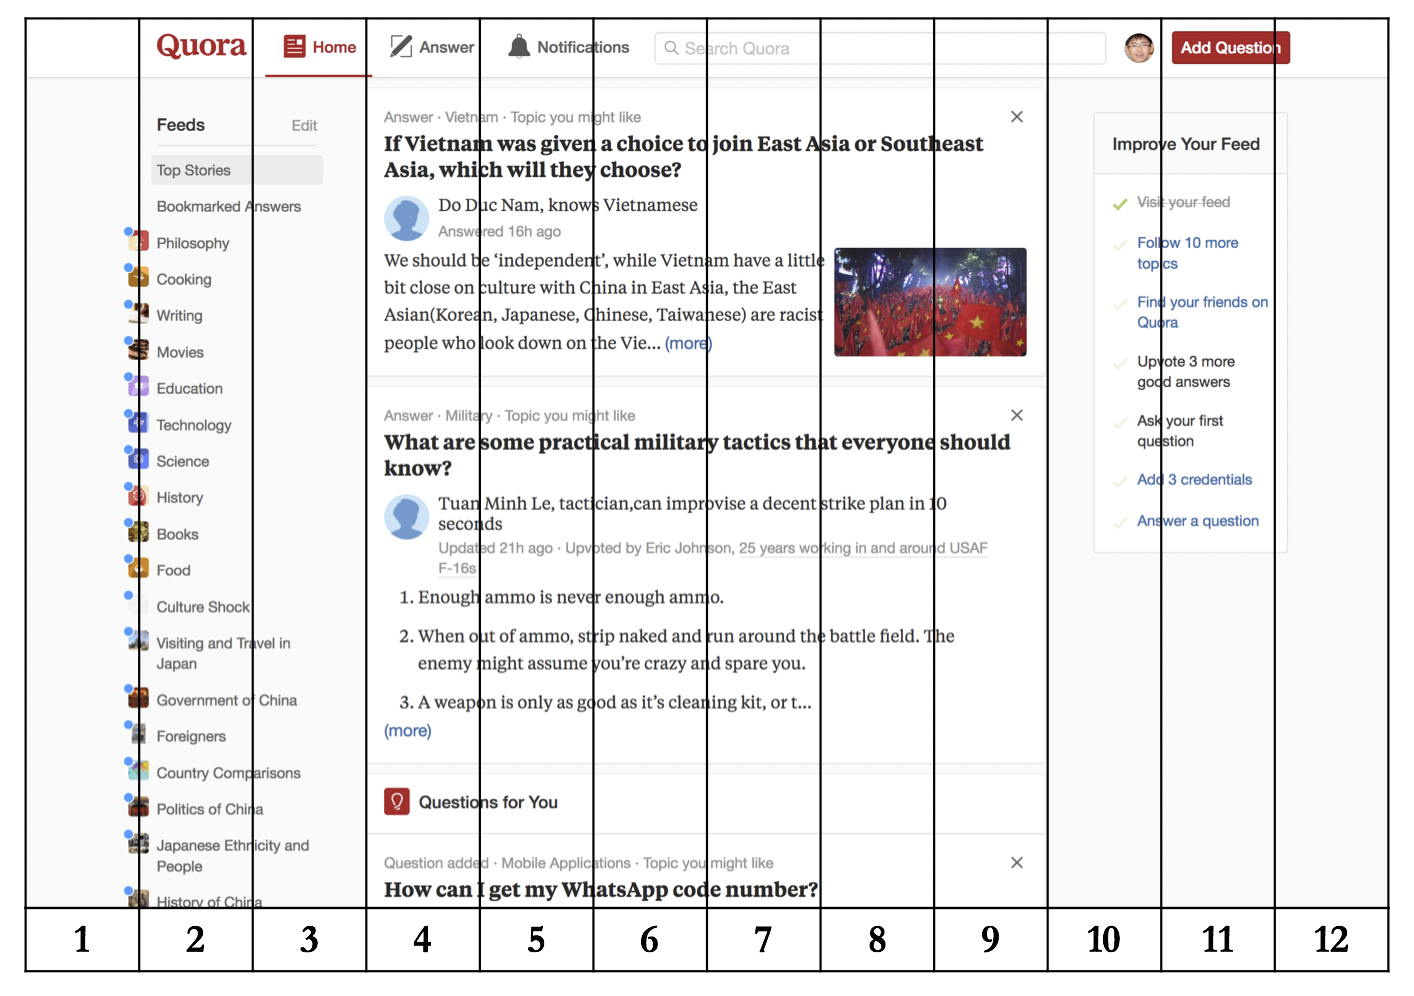
\includegraphics[width=0.95\linewidth]{quora-12}
\end{center}
\end{frame}

\begin{frame}
\frametitle{Building your own personal webpage}

\includegraphics[width=\linewidth]{website}
\end{frame}

\begin{frame}
\frametitle{Layouting (1/4)}
\begin{center}
	\begin{tabular}{|c|c|c|}
		\hline
		\multicolumn{3}{|c|}{Banner} \\ \hline
		\shortstack{Division 1 \\ (About me)} & \shortstack{Division 2 \\ (Interests)} & \shortstack{Division 3 \\ (Favourite Games)} \\ \hline
		\multicolumn{3}{|c|}{Footer} \\ \hline
	\end{tabular}
\end{center}
\end{frame}


\begin{frame}[fragile]
\frametitle{Layouting (2/4)}
\begin{center}
	\begin{tabular}{|c|c|c|}
		\hline
		\multicolumn{3}{|c|}{\mintinline{HTML}{<div class="jumbotron"></div>}} \\ \hline
		\shortstack{Division 1 \\ (About me)} & \shortstack{Division 2 \\ (Interests)} & \shortstack{Division 3 \\ (Favourite Games)} \\ \hline
		\multicolumn{3}{|c|}{Footer} \\ \hline
	\end{tabular}
\end{center}
\end{frame}

\begin{frame}[fragile]
\frametitle{Layouting (3/4)}
\begin{center}
	\begin{tabular}{|p{3.5cm}|p{3.5cm}|p{3.5cm}|}
		\hline
		\multicolumn{3}{|c|}{\mintinline{HTML}{<div class="jumbotron"></div>}} \\ \hline
		\multicolumn{3}{|c|}{\mintinline{HTML}{<div class="col-md-4"></div>} x3} \\ \hline
		\multicolumn{3}{|c|}{Footer} \\ \hline
	\end{tabular}
\end{center}
\end{frame}

\begin{frame}[fragile]
\frametitle{Layouting (4/4)}
\begin{center}
	\begin{tabular}{|p{3.5cm}|p{3.5cm}|p{3.5cm}|}
		\hline
		\multicolumn{3}{|c|}{\mintinline{HTML}{<div class="jumbotron"></div>}} \\ \hline
		\multicolumn{3}{|c|}{\mintinline{HTML}{<div class="col-md-4"></div>} x3} \\ \hline
		\multicolumn{3}{|c|}{\mintinline{HTML}{<footer></footer>}} \\ \hline
	\end{tabular}
\end{center}
\end{frame}

\section{Closing}
\subsection{Conclusion}
\begin{frame}
\frametitle{Conclusion}
\begin{center}
	\textbf{HTML} structures web pages
	
	\textbf{CSS} prettifies them
	
	\textbf{Bootstrap} makes it easier
\end{center}
\end{frame}

\begin{frame}
\frametitle{Talk to us!}
\begin{itemize}
	\item \textbf{Feedback form}: \url{https://tinyurl.com/hs2018-html}
	\item \textbf{Upcoming hackerschool}:
	\begin{itemize}
		\item Git
		\item HTML/CSS practice
		\item Introduction to ES6
	\end{itemize}
\end{itemize}
\end{frame}

\end{document}